\documentclass{llncs}
\usepackage{makeidx}  % allows for indexgeneration
\usepackage{hyperref}
\usepackage{graphicx}
\usepackage{todonotes}

\begin{document}

\title{Testing OWL Axioms Against RDF Facts:\\
A possibilistic approach}

\titlerunning{Testing OWL Axioms}                                       

\author{Andrea G. B. Tettamanzi\inst{1} \and Catherine Faron-Zucker\inst{1} \and Fabien Gandon\inst{2}}

\authorrunning{Andrea G. B. Tettamanzi et al.}

\institute{Univ. Nice Sophia Antipolis, I3S, UMR 7271, Sophia Antipolis, France,\\
\email{andrea.tettamanzi@unice.fr}, \email{faron@unice.fr}
\and
INRIA, Sophia Antipolis, France,\\
\email{fabien.gandon@inria.fr}}


\maketitle

\begin{abstract}
Automatic knowledge base enrichment methods rely critically on candidate axiom scoring.
The most popular scoring heuristics proposed in the literature are based on statistical inference.
We argue that such a probability-based framework is not always completely satisfactory
and propose a novel, alternative scoring heuristics expressed in terms of possibility theory,
whereby a candidate axiom receives a bipolar score consisting of a degree of possibility
and a degree of necessity.
We evaluate our proposal by applying it to the problem of testing \textsf{SubClassOf}
axioms against the DBpedia RDF dataset.

\keywords{ontology learning, open-world assumption, possibility theory}
\end{abstract}

\section{Introduction}
A common approach to the semantic Web puts strong emphasis
on a principled conceptual analysis of a domain of interest
leading to the construction or reuse of ontologies
as a prerequisite step for the organization of the Linked Open Data (LOD),
much like a database schema must be designed before a database can be populated.
However this approach has some limitations:
it is aprioristic and dogmatic in the way knowledge should be organized;
while it is quite successful when applied to specific domains,
it does not scale well to more general settings;
it does not lend itself to a collaborative effort; etc.
That is why an alternative, bottom-up, \emph{grass-roots} approach to ontology and
knowledge base creation better suits many scenarii: instead of postulating an \emph{a priori}
conceptualization of reality (i.e., an ontology) and requiring that our knowledge
about facts complies with it, one can start from RDF facts and learn OWL~2 axioms.

Recent contributions towards the automatic creation of OWL~2 ontologies
from large repositories of RDF facts include
FOIL-like algorithms for learning concept definitions~\cite{FanizziDAmatoEsposito2008},
statistical schema induction via association rule mining~\cite{FleischhackerVoelkerStuckenschmidt2012},
and light-weight schema enrichment methods based on the DL-Learner
framework~\cite{HellmannLehmannAuer2009,BuehmannLehmann2012}.
All these methods apply and extend techniques developed within inductive logic programming
(ILP)~\cite{ILPat20}.

On a related note, there exists a need for evaluating and validating ontologies,
be they the result of an analysis effort or of a semi-automatic learning method.
This need is witnessed by general methodological investigations
\cite{GangemiCatenacciCiaramitaLehmann2005,GangemiCatenacciCiaramitaLehmann2006}
and surveys \cite{TartirBudakArpinarSheth2007} and tools like OOPS! \cite{PovedaSuarezGomez2012}
for detecting pitfalls in ontologies.

%Ontology engineering methodologies, such as METHONTOLOGY~\cite{FernandezGomezJuristo1997},
%distinguish two validation activities, namely verification (through formal methods, syntax, logics, etc.)
%and validation through usage. Whilst this latter is usually thought of as user studies,
%an automatic process of validation based on RDF data would provide a cheap alternative,
%whereby the existing linked data may be regarded as usage traces that can be used
%to test and improve the ontologies, much like log mining can be used to provide
%test cases for development in the replay approaches.
%Alternatively, one may regard the ontology as a set of integrity constraints and check if the
%data satisfy them, using a tool like Pellet integrity constraint validator (ICV),
%which translates OWL ontologies into SPARQL queries to automatically validate RDF data~\cite{SirinTao2009}.
%A similar approach also underlies the idea of test-driven evaluation of linked data 
%quality~\cite{KontokostasWestphalAuerHellmannLehmannCornelissen2014}.
%To this end, OWL ontologies are interpreted under the closed-world assumption and
%the weak unique name assumption. 

%Yet this validation process may be seen from a reverse point of view:
%instead of starting from the \emph{a priori} assumption that a given ontology
%is correct and verify whether the facts contained in an RDF base satisfy it,
%one may treat ontologies like hypotheses and develop a methodology to verify
%whether the RDF facts corroborate or falsify them. Ontology learning and validation
%are thus strictly related.
%They could even be seen as an agile and test-driven approach to ontology development,
%where the linked data is used as a giant test case library not only to validate the
%schema but even to suggest new developments.

Ontology learning and validation rely critically on (candidate) axiom scoring.
In this paper, we will tackle the problem of testing a single, isolated axiom,
which is anyway the first step to solve the problem of validating an entire ontology.
Furthermore, to keep things reasonably simple, we will restrict our attention
to subsumption axioms of the form $\mathsf{SubClassOf}(C\ D)$.

The most popular scoring heuristics proposed in the literature are based on statistical inference.
We argue that such a probability-based framework is not always completely satisfactory.
We will propose an axiom scoring heuristics based on a formalization in possibility theory of
the notions of logical content of a theory and of falsification, loosely inspired
by Karl Popper's approach to epistemology. Our research question is: ``Can we apply
a possibilistic approach to the task of testing candidate axioms for ontology learning?''.
In addition, ``Could this be beneficial to ontology and knowledge base validation?''.


The paper is organized as follows:
Section~\ref{possibility-theory} proposes a heuristics based
on possibility theory, alternative to probability-based scoring heuristics.
Its implementation is detailed in
Section~\ref{OWL2SPARQL} and an evaluation is provided in Section~\ref{evaluation}.
Section~\ref{conclusion} draws some conclusions.

% \section{Probability-Based Candidate Axiom Scoring}
\section{A Possibilistic Candidate Axiom Scoring Heuristics}
\label{possibility-theory}

Let $\phi$ be a candidate axiom and $u_\phi$ the support or sample size for $\phi$,
i.e., the cardinality of the set of its logical consequences that will be tested in the RDF repository.
Notice that every formula which logically follows from an axiom is both
a potential falsifier (if it is contradicted by facts)
and a potential confirmation (if it is verified by facts) for that axiom.

Let $u_\phi^+$ the number of such consequences which are true (confirmations), and
$u_\phi^-$ the number of such consequences which are false (counterexamples).
A few interesting properties of these three cardinalities are:
\begin{eqnarray}
  u_\phi^+ + u_\phi^- &\leq& u_\phi;\label{eq:conf-pls-expt-lt-refc} \\
  u_\phi^+ = u_{\neg\phi}^-, \quad
  u_\phi^- &=& u_{\neg\phi}^+, \quad
  u_\phi = u_{\neg\phi}.
\end{eqnarray}

A statistics-based heuristics for the scoring of candidate axioms used
in the framework of knowledge base enrichment~\cite{BuehmannLehmann2012}
may be regarded essentially as scoring an axiom by an estimate of the probability
that one of its logical consequences is confirmed (or, alternatively, falsified)
by the facts stored in the RDF repository.
As B\"uhmann and Lehmann point out~\cite{BuehmannLehmann2012},
estimating the probability of confirmation of axiom $\phi$ just by $\hat{p}_\phi = u_\phi^+/u_\phi$
would be too crude and would not take the magnitude of $u_\phi$ into account.
That is why they base their probabilistic score on Agresti and Coull's binomial proportion
confidence interval~\cite{AgrestiCoull1998}.

One problem with such approaches is that they only look for confirmations of $\phi$
and treat their absence as failures in the calculation of the confidence interval.
This is like making an implicit closed-world assumption.
An easy fix, in view of the open-world assumption, might be, for example, to use
$\hat{p}^* = u_\phi^+/(u_\phi^+ + u_\phi^-)$ as the sample proportion instead of $\hat{p}$.

A more serious problem, however, is that these approaches rely on the assumption
that it is possible to estimate the probability that an axiom $\phi$ is true given
some evidence $e$, where $e$ = ``$\psi$ such that $\phi\models\psi$ is in the RDF repository'',
or $e$ = ``$\psi$ such that $\psi\models\neg\phi$ is in the RDF repository'',
or $e$ = ``$\psi$ such that $\phi\models\psi$ is \emph{not} in the RDF repository'', etc.,
which, by Bayes' formula, may be written as
\begin{equation}\label{eq:Bayes}
  \Pr(\phi \mid e) = \frac{\Pr(e \mid \phi)\Pr(e)}{\Pr(e \mid \phi)\Pr(e) + \Pr(e \mid \neg\phi)\Pr(\neg e)}.
\end{equation}
Therefore, in order to compute (or estimate) such probability, one should be able
to estimate the probabilities on the right-hand side of Equation~\ref{eq:Bayes}.
%such as
%\begin{itemize}
%\item the probability that a fact confirming $\phi$ is added to the repository
%  given that $\phi$ holds;
%\item the probability that a fact contradicting $\phi$ is added to the repository
%  in error, i.e., given that $\phi$ holds;
%\item the probability that a fact confirming $\phi$ is added to the repository
%  in error, i.e., given that $\phi$ does not hold;
%\item the probability that a fact contradicting $\phi$ is added to the repository
%  given that $\phi$ does not hold.
%\end{itemize}
Now, this is possible only under the (strong) assumption that the data at hand
are representative.
%Let us take a subsumption axiom $\mathsf{SubClassOf}(C\ D)$
%as an example. A fact confirming it is $D(a)$, with $C(a)$ in the dataset,
%whereas a fact contradicting it is $E(a)$, with $C(a)$ in the dataset
%and $\mathsf{DisjointClasses}(E\ D)$ in the ontology.
%Assuming that $\mathsf{SubClassOf}(C\ D)$ holds, we may suspect that
%$D(a)$ is more likely to be found in the repository
%if $D$ is either very specific (and thus ``closer'' to $a$ or very general (like
%\textsf{foaf:Person}), and less likely if it is somewhere in the middle.
%This supposition is based on our expectations of what people are likely to say
%about $a$. For instance, an average person, if asked ``what is this?'' when pointing
%to a basset hound, is more likely to answer ``a dog'' or ``an animal'' than,
%say, ``a carnivore'' or ``a mammal'', which, on purely logical grounds,
%would be perfectly valid things to say about it~\cite{Lakoff1987}.
%There is thus an inherent difficulty with estimating the above probabilities,
%one which cannot be solved otherwise than by performing a large number of
%experiments, whose results, then, would be hard to generalize.

%Another key argument for rejecting a probabilistic approach in the specific context of axiom induction from an RDF dataset like DBpedia is that this dataset contains facts automatically extracted from Wikipedia,
%which is the result of a collaborative effort, whose coverage is not planned and
%subject to cultural and historical biases.\footnote{For example, at the level
%of pop music, the coverage of DBpedia is very much biased towards anglophone artists.
%Even in domains, such as geographical data, which one would expect to be much more
%uniform and extensive, it turns out that the coverage of Wikipedia is far from being uniform.}
%Therefore, there is no reason to assume that the facts contained in an RDF triple store
%be \emph{representative} of all possible facts that could be recorded, unless
%that RDF store is the result of a planned and well-designed effort aimed at building
%a knowledge base providing uniform coverage of a given domain.
%Indeed, to use the number of facts supporting a hypothesis
%to estimate its probability one would have to make the very strong assumption
%that the finite set of facts in the RDF store is a representative sample
%of the infinite set of all ``real'' facts, whatever this means.
%Adopting a probabilistic approach whereas its assumptions are not
%fulfilled might lead to fallacious results.

To capture the basic intuition behind the process of axiom discovery without
making unwarranted assumptions, we propose an alternative axiom scoring heuristics
based on possibility theory, which is weaker than probability theory.

\subsection{Possibility Theory}
\label{PossibilityTheory}

Possibility theory \cite{Zadeh1978} is a mathematical theory of epistemic uncertainty.
Given a finite universe of discourse $\Omega$, whose elements $\omega\in\Omega$
may be regarded as events, values of a variable, possible worlds, or states of affairs,
a possibility distribution is a mapping $\pi: \Omega \to [0, 1]$,
which assigns to each $\omega$ a degree of possibility ranging from 0 (impossible,
excluded) to 1 (completely possible, normal).
A possibility distribution for  which there exists a completely possible state of
affairs ($\exists \omega^*: \pi(\omega^*) = 1$) is said to be \emph{normalized}.

There is a similarity between possibility distribution and probability 
density. However, it must be stressed that $\pi(\omega) = 1$ just means that
$\omega$ is a plausible (normal) situation and therefore should not be excluded.
A degree of possibility can then be viewed as an upper bound of a degree of probability.
Possibility theory is suitable to represent incomplete knowledge while 
probability is adapted to represent random and observed phenomena. 
We invite the reader to see~\cite{dubois1991} for more informations
about the relationships between fuzzy sets, possibility, and probability 
degrees.

A possibility distribution $\pi$ induces a \emph{possibility
measure}\index{possibility measure} and its dual \emph{necessity
measure}\index{necessity measure}, denoted by $\Pi$ and $N$
respectively. Both measures apply to a set $A \subseteq\Omega$ (or to a
formula $\phi$, by way of the set of its models, $A = \{\omega : \omega \models \phi\}$),
and are defined as follows:
\begin{eqnarray}
  \Pi(A) &=& \max_{\omega\in A} \pi(\omega); \\
  N(A)   &=& 1 - \Pi(\bar{A}) = \min_{\omega\in \bar{A}} \{1 - \pi(\omega)\}.
\end{eqnarray}
A few properties of possibility and necessity measures 
induced by a normalized possibility distribution on a finite universe of
discourse $\Omega$ are the following. For all subsets $A\subseteq \Omega$,
\begin{enumerate}
%  \item $\Pi(A \cup B) = \max\{\Pi(A), \Pi(B)\}$;
%  \item $\Pi(A \cup \bar A) = \max\{\Pi(A), \Pi(\bar A)\}=1$;
  \item $\Pi(\emptyset) = N(\emptyset) = 0$,\quad $\Pi(\Omega) = N(\Omega) = 1$;
%  \item $N(A \cap B) = \min\{N(A), N(B)\}$;
  \item $\Pi(A) = 1 - N(\bar{A})$ (duality);
%  \item $N(A) \leq \Pi(A)$;
  \item $N(A) > 0$ implies $\Pi(A) = 1$,\quad $\Pi(A) < 1$ implies $N(A) = 0$.
\end{enumerate}
In case of complete ignorance on $A$, $\Pi(A) = \Pi(\bar{A}) = 1$.

\subsection{Support of an Axiom}
\label{support}

At the beginning of this section, we have introduced the notion of support or sample
for a candidate axiom $\phi$ as the number of its logical consequences that will be
tested in the RDF repository. We shall now define that notion more precisely.

Let $\mathrm{BS}$ be a finite set of \emph{basic statements}, i.e.,
assertions, like the ones contained in an RDF repository,
that may be tested by means of a SPARQL \texttt{ASK} query.
We define the \emph{content} of an axiom $\phi$ that we wish to evaluate
as the set of its logical consequences, but we restrict it to basic statements, 
to ensure finiteness and testability:
\begin{equation}\label{eq:content}
  \mathrm{content}(\phi) = \{\psi : \phi \models \psi\} \cap \mathrm{BS}.
\end{equation}
The cardinality of $\mathrm{content}(\phi)$ is finite, because $\mathrm{BS}$ is finite,
and every formula $\psi \in \mathrm{content}(\phi)$ may be tested, because it is a basic statement.
Now we can define the support of $\phi$ as the cardinality of $\mathrm{content}(\phi)$:
\begin{equation}\label{eq:content2}
    u_\phi = |\mathrm{content}(\phi)|.
\end{equation}
%\noindent
%For the axiom $C \sqsubseteq D$, $u_{C \sqsubseteq D} = |C^\mathcal{I}|$.


\subsection{Possibility and Necessity of an Axiom}

The basic principle for establishing the possibility of a formula $\phi$ should be
that the absence of counterexamples to $\phi$ in the RDF repository means $\Pi(\phi) = 1$,
i.e., that $\phi$ is completely possible.

A hypothesis should be regarded as all the more
\emph{necessary} as it is explicitly supported by facts and not contradicted by any fact;
and all the more \emph{possible} as it is not contradicted by facts.
In other words, given hypothesis $\phi$, $\Pi(\phi) = 1$ if no counterexamples are found; 
as the number of counterexamples increases, $\Pi(\phi) \to 0$ strictly monotonically;
$N(\phi) = 0$ if no confirmations are found; as the number of confirmations increases
and no counterexamples are found, $N(\phi) \to 1$ strictly monotonically.
Notice that a confirmation of $\phi$ is a counterexample of $\neg\phi$
and that a counterexample of $\phi$ is a confirmation of $\neg\phi$.
Furthermore, the first counterexamples found to an axiom should determine a sharper decrease
of the degree to which we regard the axiom as possible than any further counterexamples,
because these latter will only confirm our suspicions and, therefore, will provide
less and less information and, similarly, in the absence of counterexamples,
the first confirmations found to an axiom should determine a sharper increase
of the degree to which we regard the axiom as necessary than any further confirmations,
because these latter will only add up to our acceptance and, therefore, will provide
less and less information.

A definition of $\Pi$ and $N$ which captures the above intuitions, but by no means
the only possible one, is, for $u_\phi > 0$,
\begin{eqnarray}
  \Pi(\phi) &=& 1 - \sqrt{1 - \left(\frac{u_\phi - u_\phi^-}{u_\phi}\right)^2}; \\
  N(\phi) &=& \sqrt{1 - \left(\frac{u_\phi - u_\phi^+}{u_\phi}\right)^2}\quad
    \mbox{if $\Pi(\phi) = 1$, 0 otherwise.}
\end{eqnarray}
Notice that this definition satisfies the duality of possibility and necessity,
in that $N(\phi) = 1 - \Pi(\neg\phi)$ and $\Pi(\phi) = 1 - N(\neg\phi)$.
%As a matter of fact, we will seldom be interested in computing the necessity and
%possibility degrees of the negation of OWL~2 axioms, for the simple reason that, in most cases,
%the latter are not OWL~2 axioms themselves. For instance, while $C \sqsubseteq D$
%is an axiom, $\neg(C \sqsubseteq D) = C \not\sqsubseteq D$ is not.

We combine the possibility and necessity of an axiom to define
a single handy acceptance/rejection index (ARI) as follows:
\begin{equation}\label{eq:ARI}
  \mathrm{ARI}(\phi) = N(\phi) - N(\neg\phi) = N(\phi) + \Pi(\phi) - 1 \in [-1, 1].
\end{equation}
A negative $\mathrm{ARI}(\phi)$ suggests rejection of $\phi$ ($\Pi(\phi)<1$),
whilst a positive $\mathrm{ARI}(\phi)$ suggests its acceptance ($N(\phi)>0$),
with a strength proportional to its absolute value. A value close to zero
reflects ignorance about the status of $\phi$.

\section{A Framework for Candidate Axiom Testing}
\label{OWL2SPARQL} 
We refer to the model-theoretic semantics of OWL~2  (as defined in \cite{OWL2-direct-semantics}),
which defines an interpretation $\mathcal{I}$ with a valuation function
$\cdot^\mathcal{I}$ mapping OWL~2 expressions into
elements and sets of elements of an interpretation domain $\Delta^\mathcal{I}$.
We take the set of all the resources that occur in a given RDF store 
as $\Delta^\mathcal{I}$ and checking an axiom amounts to checking
whether $\mathcal{I}$ is a model of the axiom. Also, calling linked data search engines
like Sindice could virtually extend the interpretation domain to the whole LOD cloud.

However, unlike interpretation domains, RDF stores are incomplete and
possibly noisy. The open-world hypothesis must be made; therefore, absence of
supporting evidence does not necessarily contradict an axiom, and an axiom might
hold even in the face of a few counterexamples (exceptions or possible mistakes).
For example, out of 541 axioms of the form $\mathsf{SubClassOf}(C\ D)$ in the DBpedia
ontology, 143 have an empty content (i.e., class $C$ is empty)
and 28 have at least one counterexample in DBpedia 3.9.\footnote{And one, namely
\textsf{SubClassOf}(\textsf{dbo:Person} \textsf{dbo:Agent}), even has 76 counterexamples!}

%The semantics of the 32 axiom types of OWL~2 may be taken as a starting point to define,
%for each axiom type, which facts recorded in a given RDF triple store are to be taken as
%supporting evidence, or \emph{confirmations} of the axiom and which facts are to be
%construed as refuting evidence, or \emph{counterexamples}, based on the principles
%laid out in Section~\ref{epistemology}.

A general algorithm for testing all the possible OWL~2 axioms in a given RDF store is beyond the scope of this paper. 
Here, we will restrict our attention to atomic class expressions and \textsf{ObjectComplementOf}
expressions, needed to test \textsf{SubClassOf} axioms.
The model-theoretic semantics of expressions of the form $\mathsf{ObjectComplementOf}(C)$
($\neg C$ in description logics syntax), where $C$ denotes a concept expression
(called \emph{class expression} in OWL~2) is $\Delta^\mathcal{I} \setminus C^\mathcal{I}$.
%Cath: le paragraphe ci-dessus est trop restrictif je pense: ce framework conviendra pour tester d'autres axiomes


Now, let us define a mapping $Q(E, x)$ from OWL~2 expressions to SPARQL graph patterns,
where $E$ is an OWL~2 expression, $x$ is a formal parameter which can be replaced by
a SPARQL variable or an RDF term,
%and match a resource identifier, or a literal,
%Cath est-ce qu'il n'y aurait pas des as où on veut pouvoir matcher des blank nodes dans le cas général?
such that the query
\texttt{SELECT DISTINCT ?x WHERE \{} $Q(E, \mbox{\tt ?x})$ \texttt{\}}
returns all the known instances of class expression $E$, which we will denote by
$[Q(E, x)]$, i.e., the equivalent of $E^\mathcal{I}$,
and the query $\mbox{\tt ASK \{ } Q(E, a) \mbox{\tt\ \}}$ checks whether $E(a)$
is in the RDF base.

For an atomic concept $A$, $Q(A, \mbox{\tt ?x}) = \mbox{\tt ?x a }A$,
where $A$ is a valid IRI.
For concept negation, things are slightly more complicated, for RDF does not support
negation.
The obvious definition
\begin{equation}\label{eq:neg-as-failure}
  Q(\neg C, \mbox{\tt ?x}) =
    \mbox{\tt \{ ?x ?p ?o . FILTER NOT EXISTS } Q(C, \mbox{\tt ?x}) \mbox{\tt\ \}},
\end{equation}
has the problem of treating negation as failure, like in databases,
where the closed-world assumption is made. 
Since we want to get as close as possible to an open-world semantics, $Q(\neg C, x)$ should be defined
differently, as the union of the concepts that are disjoint from $C$.
One might try to express this as the set of individuals $x$ that are instances of a
concept $C'$ such that no individual $z\in C^\mathcal{I}$ is an instance of $C'$,
yielding the query
\begin{equation}\label{eq:approx-open-world-negation}
  Q(\neg C, \mbox{\tt ?x}) =
  \begin{minipage}[t]{5in}
    \begin{tabbing}
      \quad\=\quad\=\quad\=\kill
      \{\>\texttt{?x a ?dc .}\\
        \>\texttt{FILTER NOT EXISTS} \{ \texttt{?z a ?dc . } $Q(C, \mbox{\tt ?z})$ \texttt{\} \}},
    \end{tabbing}
  \end{minipage}
\end{equation}
where \texttt{?z} is a variable that does not occur anywhere else in the query.
This translation is conceptually more satisfactory than the one in Equation~\ref{eq:neg-as-failure},
but it just pushes the problem one step further, because this way of testing whether
two concepts are disjoint is based on negation as failure too.
The only way to be certain that two classes are disjoint would be to find an axiom to
this effect in the ontology:
\begin{equation}\label{eq:negation-with-disjointWith}
  Q(\neg C, \mbox{\tt ?x}) =
    \mbox{\tt \{ ?x a ?dc . ?dc owl:disjointWith }
    C \mbox{\tt\ \}},
\end{equation}
otherwise, either we find an individual which is an instance of both classes,
and thus we know the two classes are not disjoint, or we don't,
in which case the two classes may or may not be disjoint.
The fact is, very few \textsf{DisjointClasses} axioms are currently found in existing
ontologies. For example, in the DBpedia ontology, the query
\texttt{SELECT ?x ?y \{ ?x owl:disjointWith ?y \}} executed on November 22, 2013
returned 17 solutions only.

\begin{figure}[t!]
  \begin{center}
    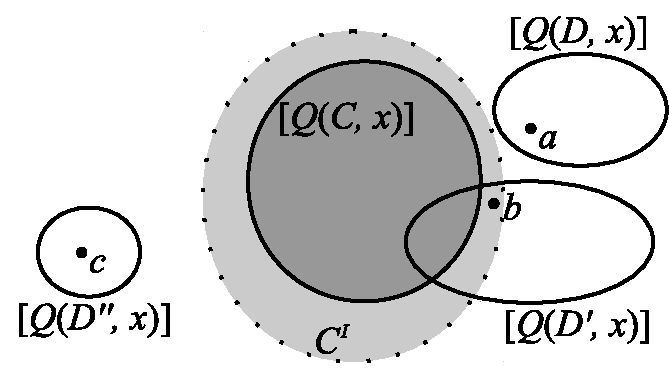
\includegraphics[height=1.2in]{../negation}
  \end{center}
  \caption{A schematic illustration of the heuristics used to capture negation
    under the open world assumption. $D''$ is a concept which is declared to
    be disjoint with $C$ in the RDF repository.\label{fig:negation}}
\end{figure}

To compare these three alternative definitions of $Q(\neg C, \mbox{\tt ?x})$,
we may refer to the diagram in Figure~\ref{fig:negation}. We wish to estimate
the actual extent of $(\neg C)^\mathcal{I}$. Clearly, $Q(C, \mbox{\tt ?x})$
(in dark grey) underestimates the real extent of $C^\mathcal{I}$ (in light gray).
Therefore, we may say that Equation~\ref{eq:neg-as-failure} overestimates
the real extent of $(\neg C)^\mathcal{I}$,
in the sense that it will regard as instances of $\neg C$ all individuals $a$
for which ``$a \mbox{\tt\ a } C$'' is not found in the RDF repository.

Now, if $b$ is such that ``$b \mbox{\tt\ a } C$'' is not known, but ``$b \mbox{\tt\ a } D'$''
is known for some class $D'$ and some instances of $D$ are known to be also
instances of $C$, then it might well be that $b$ is an instance of $C$ as well.
If, however, $a$ is such that ``$a \mbox{\tt\ a } C$'' is not known and
no instance of $D$ is known that is also an instance of $C$, then we are more
likely to believe that $a$ is not an instance of $C$.
Therefore Equation~\ref{eq:approx-open-world-negation} regards as instances of $\neg C$
fewer individuals, those for which it is highly likely that they do not belong
in $C$.

On the other hand, Equation~\ref{eq:negation-with-disjointWith} certainly underestimates
$(\neg C)^\mathcal{I}$, to the point of considering it empty
if ``$D''$ \texttt{owl:disjointWith} $C$'' is not declared in the RDF repository.
Furthermore, an individual may be an instance of $\neg C$ even though it is not an instance of a class disjoint with $C$!

To sum up, Equation~\ref{eq:neg-as-failure} is too optimistic,
Equation~\ref{eq:negation-with-disjointWith} too pessimistic, and
Equation~\ref{eq:approx-open-world-negation} somewhere in the middle.
Following the old adage ``virtue stands in the middle'', adopting
Equation~\ref{eq:approx-open-world-negation} looks like a sensible choice.

We will end this section by arguing that a suitable definition of confirmation to adopt in this
framework is Scheffler and Goodman's \emph{selective confirmation} \cite{SchefflerGoodman1972},
which characterizes a confirmation as a fact not simply satisfying an axiom, but, further,
favoring the axiom rather than its contrary.
For instance, the occurence of a black raven \emph{selectively confirms} the axiom
$\mathsf{Raven} \sqsubseteq \mathsf{Black}$ because it both confirms it and fails to confirm its
negation, namely that there exist ravens that are not black. On the contrary, the observation of
a green apple does not contradict $\mathsf{Raven} \sqsubseteq \mathsf{Black}$,
but it does not disconfirm $\mathsf{Raven} \not\sqsubseteq \mathsf{Black}$
either; therefore, it does not selectively confirm $\mathsf{Raven} \sqsubseteq \mathsf{Black}$.

\section{Evaluation on Subsumption Axiom Testing}
\label{evaluation}
The semantics of subsumption axioms of the form $\mathsf{SubClassOf}(C\ D)$
($C \sqsubseteq D$ in description logic syntax) is $C^\mathcal{I} \subseteq D^\mathcal{I}$,
which may also be written $x \in C^\mathcal{I} \Rightarrow x \in D^\mathcal{I}$.
Therefore, $\mathrm{content}(C \sqsubseteq D) = \{D(a) : \mbox{$C(a)$ in the RDF store} \}$,
because, if $C(a)$ holds, $C(a) \Rightarrow D(a) = \neg C(a) \lor D(a) = \top \lor D(a) = D(a)$.
%The content of such axioms may thus be defined as
%\begin{equation}
%  \mathrm{content}(C \sqsubseteq D) = \{C(a) \Rightarrow D(a) : \mbox{$C(a)$ in the RDF store} \},
%\end{equation}
The support $u_{C \sqsubseteq D}$ of the axiom can thus be computed with the following SPARQL query:
\begin{equation}
  \begin{minipage}[c]{5in}
    \begin{tabbing}
      \quad\=\quad\=\quad\=\kill
      \texttt{SELECT (count(DISTINCT ?x) AS ?u)}
      \texttt{WHERE} \{$Q(C, \mbox{\tt ?x})$\}.
    \end{tabbing}
  \end{minipage}
\end{equation}
In order to compute $ARI(C \sqsubseteq D)$, we must provide a computational definition of $u^+_{C \sqsubseteq D}$ and $u^-_{C \sqsubseteq D}$. We start with the following statements:
\begin{itemize}
\item confirmations are individuals $i$ such that
  $i \in [Q(C, x)]$ and $i \in [Q(D, x)]$;
\item counterexamples are individuals $i$ such that
  $i \in [Q(C, x)]$ and $i \in [Q(\neg D, x)]$.
\end{itemize}
This may be translated into SPARQL queries to compute $u^+_{C \sqsubseteq D}$ and $u^-_{C \sqsubseteq D}$:
\begin{equation}
  \begin{minipage}[c]{5in}
    \begin{tabbing}
      \quad\=\quad\=\quad\=\kill
      \texttt{SELECT (count(DISTINCT ?x) AS ?numConfirmations)}\\
      \texttt{WHERE} \{ $Q(C, \mbox{\tt ?x})$ $Q(D, \mbox{\tt ?x})$ \}
    \end{tabbing}
  \end{minipage}
\end{equation}
and
\begin{equation}
  \begin{minipage}[c]{5in}
    \begin{tabbing}
      \quad\=\quad\=\quad\=\kill
      \texttt{SELECT (count(DISTINCT ?x) AS ?numCounterexamples)}\\
      \texttt{WHERE} \{ $Q(C, \mbox{\tt ?x})$ $Q(\neg D, \mbox{\tt ?x})$ \}
    \end{tabbing}
  \end{minipage}
\end{equation}
respectively.
Notice that an $i \in [Q(C, x)]$ such that $i \notin [Q(D, x)]$
does not contradict $C \sqsubseteq D$, because it might well be the case
that the assertion ``$i \mbox{\tt\ a } D$'' is just missing.
Likewise, an $i \in [Q(\neg D, x)]$ such that $i \in [Q(\neg C, x)]$
will not be treated as a confirmation, based on our choice to regard as
evidence in favor of a hypothesis only selective confirmations.

We evaluated the proposed scoring heuristics by performing tests of subsumption
axioms using DBpedia 3.9 in English as the reference RDF fact repository.
In particular, on April 27, 2014, we downloaded the DBpedia dumps of English version 3.9,
generated in late March/early April 2013, along with the DBpedia ontology, version 3.9.
This local dump of DBpedia, consisting of 812,546,748 RDF triples,
has been bulk-loaded into Jena TDB and a prototype
for performing axiom tests using the proposed method has been coded in Java,
using Jena ARQ and TDB to access the RDF repository.

All experiments have been performed on a Fujitsu CELSIUS workstation equipped
with twelve six-core Intel Xeon CPU E5-2630 v2 processors at 2.60GHz clock speed,
with 15,360 KB cache each, 128 GB RAM,
4 TB of disk space with a 128 GB SSD cache,
under the Ubuntu  12.04.4 LTS 64-bit operating system.


We performed two experiments of different type: an explorative test of systematically
generated subsumption axioms and an exhaustive test of all subsumption axioms
in the DBpedia ontology.\footnote{Results available
at URL \url{http://www.i3s.unice.fr/~tettaman/RDFMining/}.}

For the former experiment, we systematically generated and tested subsumption axioms
involving atomic classes only according the following protocol:
for each of the 442 classes $C$ referred to in the RDF repository, we construct all axioms of the form
$C \sqsubseteq D$ such that $C$ and $D$ share at least one instance. Classes $D$ are obtained
with query \texttt{SELECT DISTINCT ?D WHERE \{}$Q(C, \mbox{\tt ?x})$. \texttt{?x a ?D\}}.
Due to the sheer number of axioms thus generated, and to the long time
it takes to test them,\footnote{Up to 27 hours for axiom \textsf{SubClassOf}(\textsf{dbo:Eukaryote} \textsf{dbo:Artist})!}
this experiment could not complete at the time of writing and is still underway;
however, a sufficient number of axioms was tested to allow gathering some statistics.
Figure~\ref{fig:systematic-time}a shows the distribution of test time,
while the plot of time vs.\ ARI of axioms in Figure~\ref{fig:systematic-time}b
suggests that the time it takes to test an axiom is inversely proportional to its
ARI. This is good news, because it suggests that putting a time-out
on the test would be an acceptable heuristics to decide whether to accept or reject
a candidate axiom, for an axiom which takes too long to test will likely end up
having a very negative ARI.

\begin{figure}[t]
\begin{center}
  \begin{tabular}{cc}
    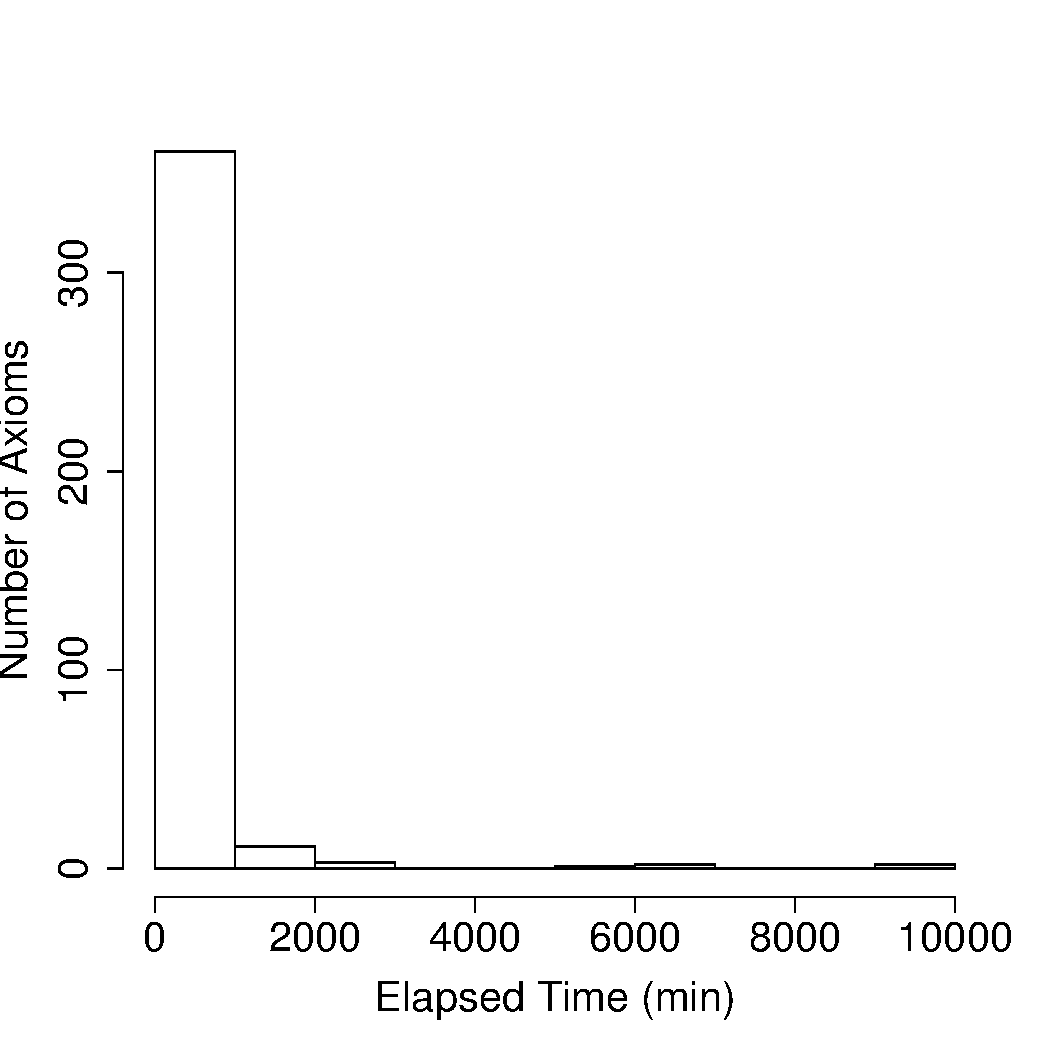
\includegraphics[height=2.25in]{systematic-time-hist} &
    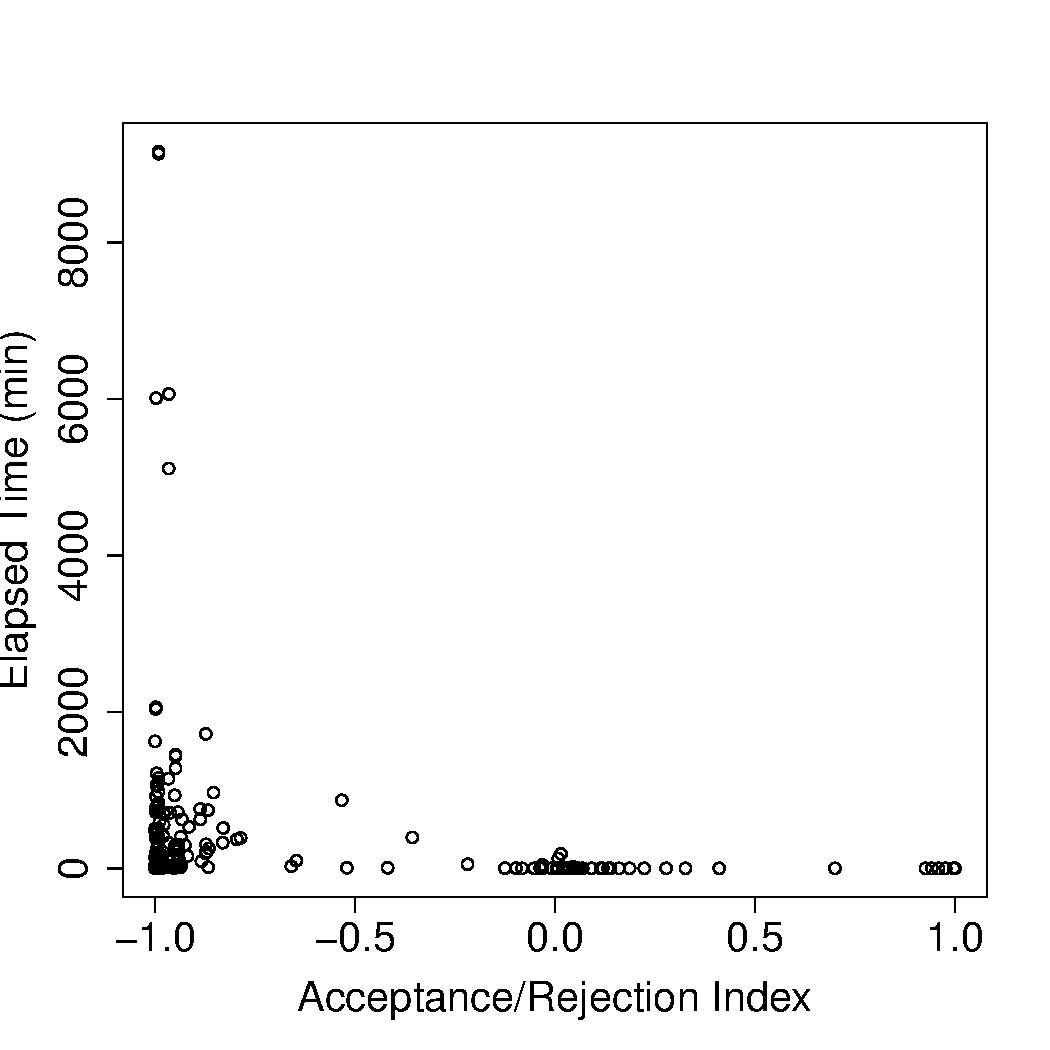
\includegraphics[height=2.25in]{time-ARI} \\
    (a) & (b)
  \end{tabular}
\end{center}
\caption{A histogram showing the distribution of test time of systematically generated
  \textsf{SubClassOf} axioms (a), and a plot of the time taken
  for testing as a function of ARI.}
\label{fig:systematic-time}
\end{figure}

By construction, all axioms generated in this experiment have at least one confirmation
and, as a consequence, non-zero possibility (thus $\mathrm{ARI} > -1$).

\begin{figure}[t]
\begin{center}
  \begin{tabular}{cc}
    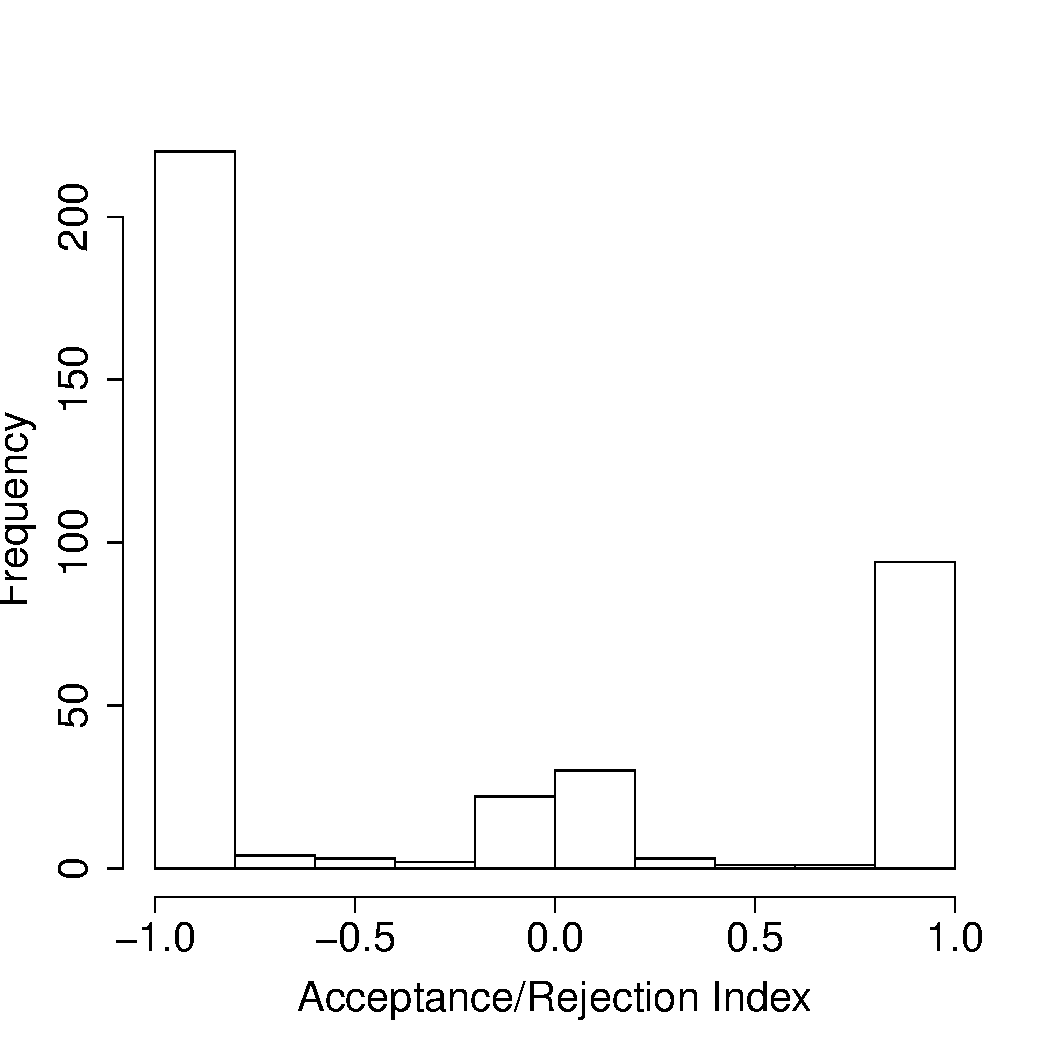
\includegraphics[height=2.25in]{ARI-hist} &
    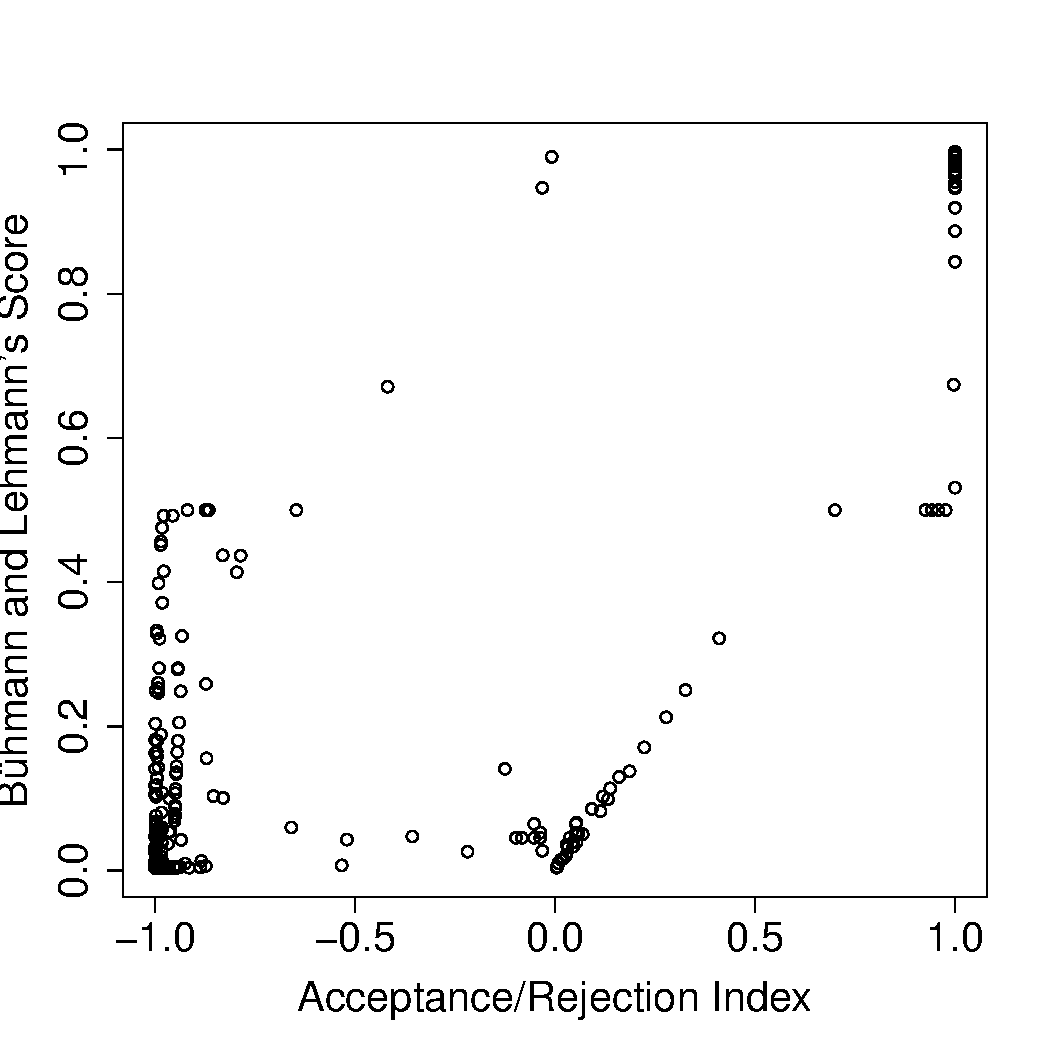
\includegraphics[height=2.25in]{ARI-BLS} \\
    (a) & (b)
  \end{tabular}
\end{center}
\caption{A histogram showing the distribution of the acceptance/rejection index
  of systematically generated \textsf{SubClassOf} axioms (a),
  and the relationship between the acceptance/rejection index and the probability-based
  score used in~\cite{BuehmannLehmann2012} (b).}
\label{fig:ARI}
\end{figure}

The ARI values of systematically generated axioms tend to cluster
around the three values $-1$, 0, and 1 (see Figure~\ref{fig:ARI}a).

To assess the discriminatory ability of the proposed scoring heuristics,
we have evaluated these results by sorting the
% UPDATE AS MORE AXIOMS ARE TESTED:
380
tested axioms by their ARI and by manually tagging each of them as either \emph{true} or \emph{false} based on common sense.
Three out of the 78 axioms with an ARI of 1 are clearly false: 
\textsf{SubClassOf(dbo:Eukaryote dbo:Species)},
\textsf{SubClassOf(dbo:OrganisationMember dbo:Sports\-TeamMember)}, and
\textsf{SubClassOf(dbo:SportCompetitionResult dbo:OlympicResult)}.
However, no scoring heuristics based on counting would be able to tell
these 3 false positives from the true ones.
Proceeding by decreasing ARI, the first false axiom encountered was
\textsf{SubClassOf(dbo:TennisLeague skos:Concept)}, with an ARI of 0.699854,\footnote{The confirmations of this and several other axioms of the form \textsf{SubclassOf($C$ skos:Concept)}
with a much lower ARI are obvious mistakes: no individual should be a
\textsf{skos:Concept}. This seems now to have been fixed in the live version of DBpedia.}
followed by the true axiom \textsf{SubClassOf(dbo:Road gml:\_Feature)},
with an ARI of 0.410399, followed by a large number of false axioms, starting with
\textsf{SubClassOf(schema:Product gml:\_Feature)} with an ARI of 0.326187.
This positive ARI means no counterexamples were found; the 2,806 confirmations are all
instances of classes \textsf{dbo:Aircraft} and \textsf{dbo:Ship} having, strangely enough, geographical coordinates.

A few seemingly true axioms are found with an ARI around zero. They are
\textsf{SubClassOf(schema:School schema:Place)},
\textsf{SubClassOf(schema:School dbo:\-Place)}, with an ARI of 0.00830433,
and
\textsf{SubClassOf(schema:School dbo:EducationalInstitu\-tion)},
\textsf{SubClassOf(schema:School dbo:Organisation)},
\textsf{SubClassOf(schema:School\break schema:EducationalOrganization)}, and
\textsf{SubClassOf(schema:School schema:Organ\-ization)}, with an ARI of $-0.00830433$.

A dubious case is
\textsf{SubClassOf(schema:Museum dbo:Building)}, with an ARI of $-0.031754$,
3,957 confirmations and two counterexamples \textsf{:Saint\_Peter's\-\_Basilica} and
\textsf{:US\_90}. We tagged it as false, because one could imagine
a museum hosted on a ship or an open-air museum, but we admit to our choice being debatable.

This distribution of true and false axioms suggests $\mathrm{ARI}(\phi)>1/3$
as the optimal acceptance criterion for a candidate axiom $\phi$.
This would yield 4 false positives and 6 false negatives (corresponding to a
% UPDATE AS MORE AXIOMS ARE TESTED:
97.37\%
accuracy).
However, it appears that the misclassification of the above axioms is to blame
on mistakes in DBpedia. This highlights the potential for the proposed heuristics
as a tool for RDF data validation: confirmations and counterexamples of axioms
with ARI around zero is where the search for bugs should focus.

It is interesting to compare these results with those one would obtain by using
a probability-based score. Figure~\ref{fig:ARI}b provides a comparison by plotting
each axiom according to its ARI (X-axis) and its score computed as in~\cite{BuehmannLehmann2012}
(Y-axis). First of all it is clear that both scores tend to agree in the extremes,
with some notable exceptions, but behave quite differently in all other cases.
The probabilistic score with the 0.7 threshold suggested by~\cite{BuehmannLehmann2012}
gives 13 false negatives (7 more than the ARI) and 4 false positives (the three
false axioms with ARI of 1, plus \textsf{SubClassOf(schema:Museum dbo:Building)},
which we tagged as false).
Among the false negatives, there are five axioms with an ARI of 1 which are
rejected by the probabilistic score: they are all of the form
\textsf{SubClassOf(dbo:TennisLeague $D$)}. Then we find
\textsf{SubClassOf(schema:School schema:Place)} and
\textsf{SubClassOf(schema:School dbo:Place)}, which were also rejected by the ARI,
and six axioms of the form \textsf{SubClassOf($C$ gml:\_Feature)}, which have
ARIs comprised between 0.41 and 0.997.
Finally, most false axiom candidates get an ARI close to $-1$, whilst their
probabilistic scores are almost evenly distributed between 0 and 0.5. We might
say that, besides being more accurate, ARI gives clearer indications than
the probabilistic score.

For the second, more validation-oriented experiment, we extracted an exhaustive
list of \textsf{SubClassOf} axioms in the DBpedia ontology, in functional syntax, with the query
\begin{verbatim}
SELECT DISTINCT concat("SubClassOf(<",str(?x),"> <",str(?y),">)")
WHERE { ?x a owl:Class . ?x rdfs:subClassOf ?y }\end{verbatim}
thus obtaining 541 axioms. Testing them took ``only'' 1 h 23 min 31 s, due to
the fact that most of these axioms have a positive ARI and can thus be tested
relatively rapidly.

%Figure~\ref{fig:time} shows the distribution of the time testing each axiom took,
%as well as a plot showing that such time tends to be proportional to the axiom's
%reference cardinality, i.e., the number of its potential falsifiers.
%Testing time appears to follow a power law: most axioms take less than a minute
%to be tested, but a few of them may even take hours.
%%cath essayer d'expliquer pourquoi et donc de couper quand le temps dépasse une limite

%\begin{figure}[t]
%\begin{center}
%  \begin{tabular}{cc}
%    \includegraphics[height=2.25in]{time-hist} &
%    \includegraphics[height=2.25in]{time-refc} \\
%    (a) & (b)
%  \end{tabular}
%\end{center}
%\caption{A histogram showing the distribution of the elapsed time for testing
%  DBpedia ontology \textsf{SubClassOf} axioms (a), and a plot of the time taken
%  for testing each individual axiom as a function of their reference cardinality.}
%\label{fig:time}
%\end{figure}

A large number of these axioms (143) turned out to have $u_\phi = 0$ (empty content)
thus their ARI is 0. For 28 axioms, a negative ARI signals the presence of
seemingly erroneous facts: the following table gives a few examples of axioms
$C \sqsubseteq D$ with their conterexamples
(instances of the subclass that also belong to a class disjoint with the superclass, i.e.,
$a$ such that $C(a)$ and $E(a)$ with $E^\mathcal{I} \cap D^\mathcal{I} = \emptyset$:
in this case, either $C(a)$ is wrong or $E(a)$ is).
\begin{center}\scriptsize
  \begin{tabular}{|l|l|} \hline
  \textbf{Axiom} & \textbf{Counterexamples} \\ \hline
\textsf{SubClassOf(dbo:LaunchPad dbo:Infrastructure)} & \textsf{:USA} \\ \hline
\textsf{SubClassOf(dbo:Brain dbo:AnatomicalStructure)} & \textsf{:Brain} [\emph{sic}] \\ \hline
\textsf{SubClassOf(dbo:Train dbo:MeanOfTransportation)} &
  \textsf{:New\_Jersey\_Transit\_rail\_op\-er\-ations}, \\
& \textsf{:ALWEG} \\ \hline
\textsf{SubClassOf(dbo:ProgrammingLanguage dbo:Software)} & \textsf{:Ajax} \\ \hline
\textsf{SubClassOf(dbo:PoliticalParty dbo:Organisation)} &
  \textsf{:Guelphs\_and\_Ghibellines}, \textsf{:-},\footnotemark \\
& \textsf{:New\_People's\_Army}, \textsf{:Syrian}\\
\hline
  \end{tabular}
\footnotetext{That is \texttt{<}\url{http://dbpedia.org/resource/-}\texttt{>}.
  This IRI is dereferenced to the ``hyphen-minus'' resource.}\end{center}

\section{Conclusion}
\label{conclusion}
We have proposed a candidate axiom scoring heuristics, based on possibility theory,
to be used for automatic axiom induction from RDF data
and, ultimately, to provide a solid basis for ontology learning.
In addition, we have developed a framework based on the proposed heuristics,
which uses the model-theoretic semantics of OWL~2 and SPARQL queries to test
candidate axioms.

The results of experimental evaluation on the DBpedia dataset clearly indicate
that the proposed heuristics is suitable for tasks such axiom
induction and ontology learning and, furthermore, may be beneficial as a tool
for ontology and knowledge-base validation.

One may object that, being based on possibility theory, our scoring heuristics
is less objective than a probability-based scoring method. However, we have argued
in Section~\ref{possibility-theory} that scoring heuristics based on probability are doomed
to be arbitrary and subjective or, in other words, \emph{qualitative}
and, therefore, hardly more rigorous or objective than the proposed approach.
The experimental results corroborate this claim.

Future work includes extending the experimental evaluation to more general sets
of candidate axioms and enlarging the test base by including additional RDF datasets
from the LOD.
We also plan on improving the implementation of the framework by setting a time-out
on query evaluation to reduce the computational overhead of axiom testing.

\bibliographystyle{tetta-lncs}
\bibliography{../RDFMining}
\end{document}

